\documentclass[../../lecture_notes.tex]{subfiles}

\begin{document}

\noindent To do computation, we must first convert from first-order logic to propositional logic.\\
In general, we do replacement, written as: \{x/y\} — replace x with y.\\
We must handle instantiation uniquely, however: \begin{enumerate} [itemsep=0mm]
	\item UNIVERSAL INSTANTIATION\\
		($\forall$ variable) (sentence) subst({variable/ground-term}, sentence)\\
		ex: for constants \{John, Richard\}:\\
		$\forall$ x King(x) $\land$ Greedy(x) $\implies$ Evil(x)\\
		$\rightarrow$ King(John) $\land$ Greedy(John) $\implies$ Evil(John)\\
		$\rightarrow$ King(Richard) $\land$ Greedy(Richard) $\implies$ Evil(Richard)\\
		$\rightarrow$ King(Father(John)) $\land$ Greedy(Father(John)) $\implies$ Evil(Father(John))\\
		While this creates ground sentences, we can see that it could run infinitely
	\item EXISTENTIAL INSTANTIATION\\
		($\exists$ variable) (sentence) subst({variable/new-constant}, sentence)\\
		ex: for constants\{C\}\\
		$\exists$ x Crown(x) $\land$ On-Head(x, John)\\
		$\rightarrow$ Crown(C) $\land$ On-Head(C, John)
\end{enumerate}
\noindent Without any functions, this term count is finite, but with functions, it could be infinite.\\
We can see that in these cases:
\begin{enumerate} [itemsep=0mm]
	\item $\forall$ level 1 = $\forall$ level 2
	\item SAT($\exists$ level 1) $\iff$ SAT($\exists$ level 2)
\end{enumerate}

\noindent This has a major result:\\
	\indent \textbf{\underline{Theorem (Herbrand 1980)}}\\
        \indent \indent if a sentence is entailed by a first order logic knowledge base,\\
        \indent \indent then it is entailed by a finite subset of that propositional knowledge base.\\
Application:\\
	\indent for n = 0 to $\infty$ do\\
	\indent \indent create a propositional knowledge base by instantiating with depth-n terms\\
	\indent \indent see if the sentence is entailed by this knowledge base\\
We have a problem, however:\\
	\indent this only terminates if the sentence is entailed!\\
	\indent $\implies$ inference is considered \textbf{\underline{semi-decidable}} (Church/Turing 1936)\\
\\
We can use resolution to prove implications as with propositional logic.\\
We must first define the idea of \textbf{\underline{unification}}.\\
A \textbf{\underline{unifier}} is a set of variable assignments that make two statements equivalent.\\
	\indent Examples:
		\begin{enumerate} [itemsep=0mm]
			\item Knows(John, x) \& Knows(John, John), \{x/John\} $\rightarrow$ Knows(John, John)
			\item Knows(John, x) \& Knows(y, OJ), \{x/OJ, y/John\} $\rightarrow$ Knows(John, OJ)
			\item Knows(John, x) \& Knows(y, Mother(y)), \{x/Mother(John), y/John\} 
				→ Knows(John, Mother(John)
			\item Knows(John, x) \& Knows(x, OJ), NO SOLUTION
		\end{enumerate}
We can improve unification by indexing facts/predicate indexing\\
	\indent $\equiv$ we cache highly used facts — very useful for many predicate, few clause logics.\\
If we store by predicate and first argument, then we can lookup by either.\\
This formed a subsumption lattice where children are formed by substitution on a higher.\\
In this lattice, the highest common descendent of two nodes comes from their MGU.\\
Since this is $O(2^n)$, it requires a small n; thankfully, most AI problems meet this.\\
\\
First order resolution goes as in the following example:\begin{align*}
	((\forall x Rich(x) \implies Unhappy(x))&, Rich(Ken))\\
	\{\neg \text{Rich(x) } \lor \text{Unhappy(x)}, &\text{Rich(Ken)}\}\\
	\frac{\neg\text{Rich(x)} \lor \text{Unhappy}(x), \text{Rich(Ken)}} {\text{Unhappy(Ken)}}& \text{ with \{x/Ken\}}
\end{align*}
We use this to walk through the following proof:\\
	\indent Statements:
		\begin{itemize} [itemsep=0mm]
			\item Jack owns a dog.
			\item Every dog owner is an animal lover
			\item No animal lover kills an animal
			\item Either Jack or curiosity killed the cat
			\item Cats are animals
		\end{itemize}
	\indent Query: Did curiosity kill the cat?\\
	\indent First Order Knowledge Base:
		\begin{itemize} [itemsep=0mm]
			\item Owns(Jack, Dog)
			\item $\forall$ x ($exists$ y Owns(x, y) $\land$ Dog(y)) $\implies$ ALover(x)
			\item $\forall$ x ALover(x) $\implies$ ($\forall$ y Animal(y) $\implies$ $\neg$kills(x, y))
			\item Kills(Jack, Tuna) $\lor$ Kills(Curiosity, Tuna)
			\item Cat(Tuna)
			\item $\forall$ x Cat(x) $\implies$ Animal(x)
		\end{itemize}
	\indent CNF Knowledge Base:
		\begin{enumerate} [itemsep=0mm]
			\item Dog(D)
			\item Owns(Jack, D)
			\item $\neg$Owns(x, y) $\lor$ $\neg$Dog(y) $\lor$ ALover(x)
			\item $\neg$ALover(x) $\lor$ $\neg$Animal(y) $\lor$ $\neg$Kills(x, y)
			\item Kills(Jack, Tuna) $\lor$ Kills(Curiosity, Tuna)
			\item Cat(Tuna)
			\item $\neg$Cat(x) $\lor$ Animal(x)
			\item Query — $\neg$Kills(Curiosity, Tuna)\\
			----------------------------------------------------------------------------------------------
			\item $\neg$Owns(x, D) $\lor$ ALover(x) by <1, 5>: {y/D}
			\item ALover(Jack) by <2, 9>: {x/Jack}
			\item Animal(Tuna) by <7, 8>: {x/Tuna}
			\item $\neg$ALover(x) $\lor$ $\neg$Kills(x, Tuna) by <4, 11>: {x/Tuna}
			\item $\neg$Kills(Jack, Tuna) by <10, 12>: {x/Jack}
			\item Kills(Jack, Tuna) by <8, 5>
			\item CONTRADICTION by <12, 13>
		\end{enumerate} \medskip

\noindent To perform resolution, we need a CNF; we convert to a CNF much the same as with propositional:
Consider: $\forall$ x [$\forall$ y Animal(y) $\implies$ Loves(x, y)] $\implies$ [$\exists$ y Loves(y, x)]\\
	\indent Step 1: eliminate $\implies$ and $\iff$\\
	\indent\indent $\forall$ x [$\neg$$\forall$ y $\neg$Animal(y) $\lor$ Loves(x, y)] $\lor$ [$\exists$ y Loves(y, x)]\\
	\indent Step 2: move negation inward\\
	\indent \indent $\forall$ x [$\exists$ y Animal(y) $\land$ $\neg$Loves(x, y)] $\lor$ [$\exists$ y Loves(y, x)]\\
	\indent Step 3: standardize variables\\
        \indent \indent $\forall$ x [$\exists$ y Animal(y) $\land$ $\neg$Loves(x, y)] $\lor$ [$\exists$ z Loves(z, x)]\\
	\indent Step 4: “skolem”-ize\\
        \indent \indent $\forall$ x [Animal(F(x)) $\land$ $\neg$Loves(x, F(x))] $\lor$ [Loves(G(x), x)]\\
	\indent Step 5: drop universal quantifiers\\
        \indent \indent [Animal(F(x)) $\land$ $\neg$Loves(x, F(x))] $\lor$ [Loves(G(x), x)]\\
	\indent Step 6: distribute\\
        \indent \indent [Animal(F(x)) $\lor$ Loves(G(x), x)] $\lor$ [$\neg$Loves(x, F(x)) $\lor$ Loves(G(x), x)]\\
\\
We have a special case when the knowledge base contains only \textbf{\underline{definite clauses}}.\\
\indent a definite clause contains exactly one positive term (ex $\neg$A $\lor$ $\neg$B $\lor$ C)\\
\indent we can thus convert these to an if-then rule (ex $A \land B \implies C$)\\
\\
We will show two special algorithms for dealing with definite clause knowledge bases.\\
We will do this with the following example:
	\begin{enumerate} [itemsep=0mm]
		\item American(x) $\land$ Weapon(x) $\land$ Sells(x, y, z) $\land$ Hostile(z) $\implies$ Criminal(x)
		\item $\exists$ x Owns(Nono, x) $\land$ Missile(x) \\
			Owns(Nono, M1) $\land$ Missile(M1)
		\item Missile(x) $\land$ Owns(Nono, x) $\implies$ sells(West, x, Nono)
		\item Missile(x) $\implies$ Weapon(x)
		\item Enemy(x, America) $\implies$ Hostile(x)
		\item American(West)
		\item Enemy(Nono, America)
	\end{enumerate}

\noindent Notice that to be operated on, all clauses must be universally quantified

\subsubsection*{Forward Chaining}
\begin{center}\begin{figure}[H]
	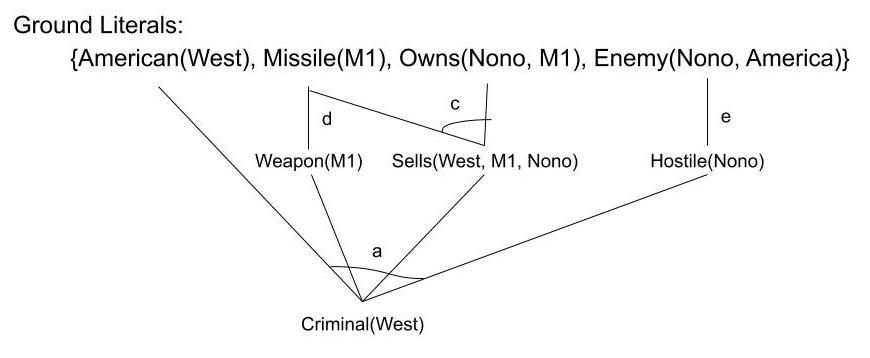
\includegraphics[scale=0.5]{forward_chain}
\end{figure}\end{center}
\noindent If there are no function symbols and all clauses are definite, the KB is a \textbf{\underline{data log}}\\
\indent These are especially conducive to representing databases.\\
If we preprocess as rules come in, we can handle many facts and even model a brain in real time.\\

\subsubsection*{Backward Chaining}
\begin{center}\begin{figure}[H]
	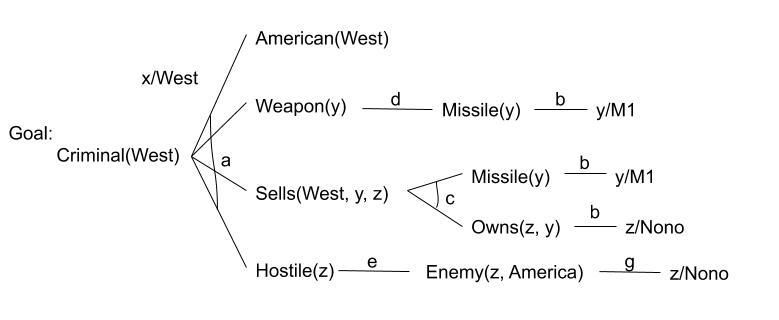
\includegraphics[scale=0.5]{backward_chain}
\end{figure}\end{center}
\noindent This is often used with improvements for logic programming (as in prolog)\\
The system often caches subgoals (like Missile(y)) for efficiency’s sake

\end{document}